\documentclass[aspectratio=169]{beamer}
\usetheme{Boadilla}
\usepackage{graphicx}
\usepackage{bookmark}
\title{Traffic Speed Prediction}
\subtitle{AML baselines and graph learning}
\author{Project presentation}
\date{\today}
\begin{document}
\begin{frame}\titlepage\end{frame}

\begin{frame}{Available measurements}
\begin{itemize}
\item METR-LA: 34,272 timestamps and 207 sensors, five-minute speed readings.
\item PEMS-BAY: 52,116 timestamps and 325 sensors, with sensor metadata.
\item Speed only: traffic flow and occupancy are not supplied.
\item Zero speed values are treated as missing observations.
\end{itemize}
\end{frame}

\begin{frame}{Forecast protocol}
\begin{itemize}
\item Chronological split: 70\% train, 10\% validation, 20\% test.
\item Forecast horizons: 5, 15, 30, and 60 minutes.
\item Inputs: recent speed lags, time-of-day, weekday, and sensor segment.
\item Compare persistence, multi-output Random Forest, pooled XGBoost, and GAT.
\item Fixed METR-LA distance graph; chronological split and masked missing targets.
\end{itemize}
\end{frame}

\begin{frame}{Held-out METR-LA MAE}
\begin{center}
\begin{tabular}{lrrrr}
\textbf{Model} & \textbf{5m} & \textbf{15m} & \textbf{30m} & \textbf{60m} \\
\hline
Persistence & 2.814 & 3.499 & 4.207 & 5.381 \\
Random Forest & \textbf{2.519} & \textbf{3.119} & \textbf{3.635} & \textbf{4.192} \\
XGBoost & 2.554 & 3.239 & 3.854 & 4.542 \\
GAT & 2.879 & 3.466 & 4.087 & 4.898
\end{tabular}
\end{center}
\IfFileExists{../results/figures/22_metr_la_backtest_metrics.png}{
\begin{center}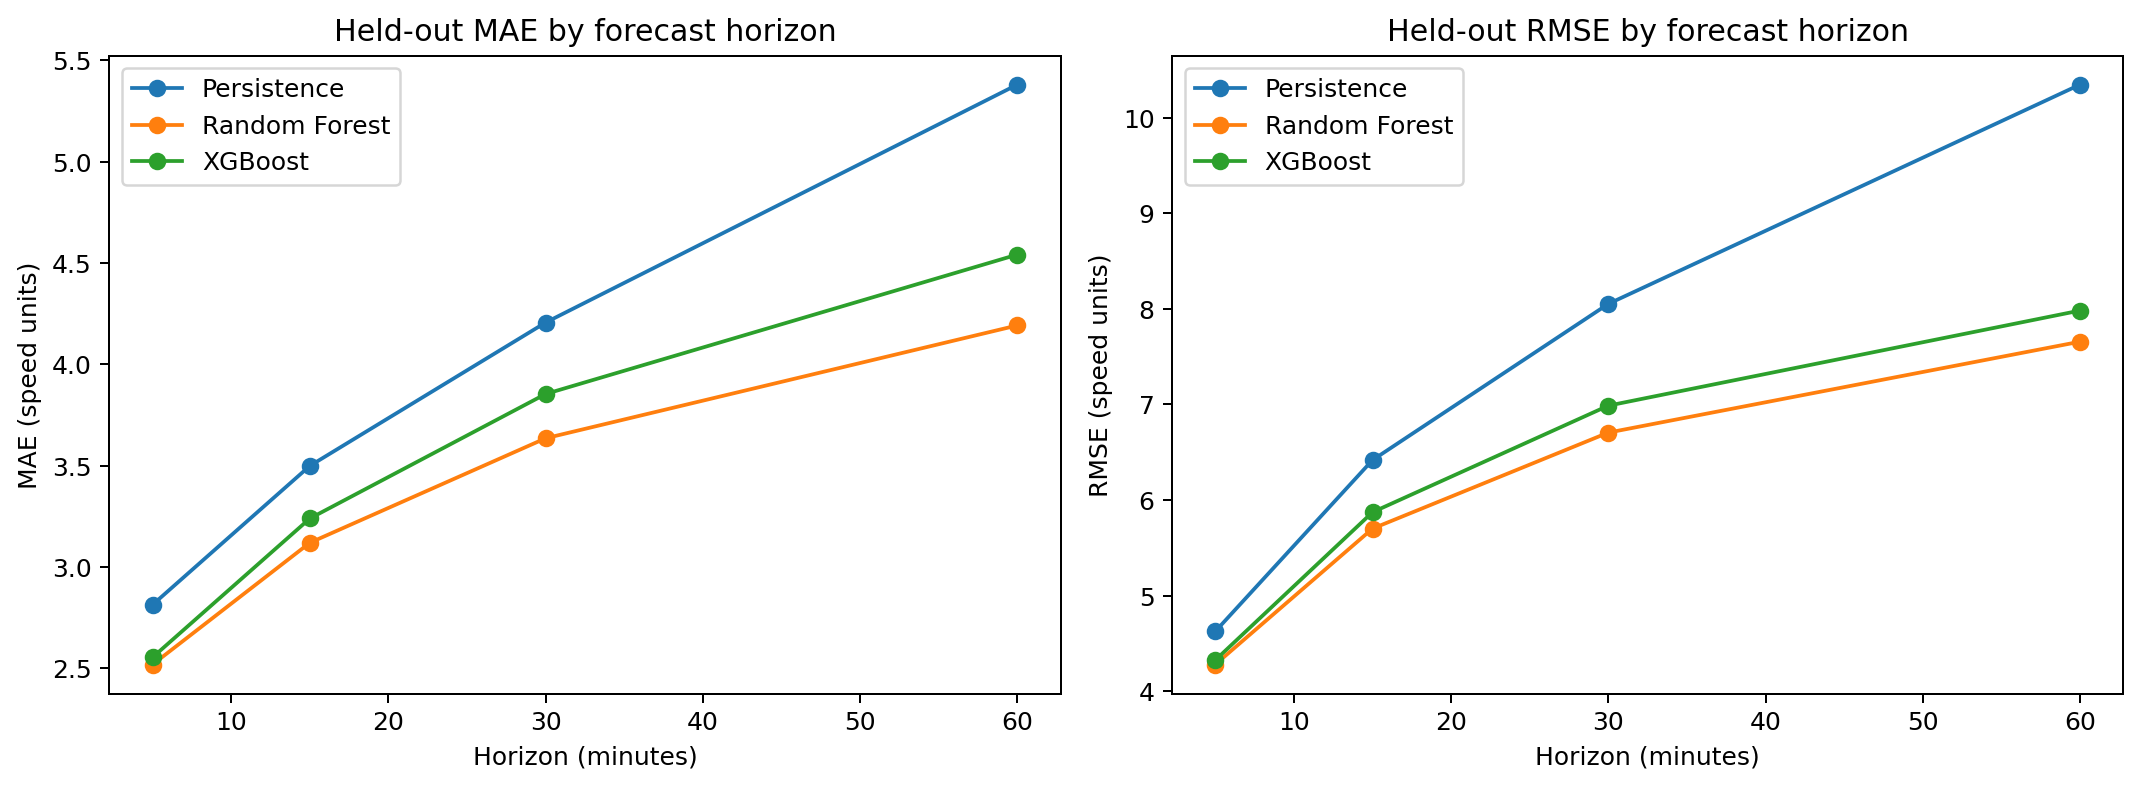
\includegraphics[height=.48\textheight]{../results/figures/22_metr_la_backtest_metrics.png}\end{center}}{}
\end{frame}

\begin{frame}{Limitations and next steps}
\begin{itemize}
\item Random Forest has the lowest overall MAE at all four horizons; GAT is trained but does not beat either tree model overall.
\item The symmetrized distance graph represents spatial proximity, not verified upstream/downstream direction.
\item Signal simulation needs traffic volumes/queues, signal phases, and timing plans.
\item Flow and occupancy are unavailable in the supplied traffic CSVs.
\item The user-supplied reference table is not represented as a reproduced result.
\end{itemize}
\end{frame}
\end{document}
